% !TEX program = pdflatex
%
% Dieses Kapitel kann entweder standalone kompiliert werden
%   (dann mit fiktiven Daten) oder in die Hauptarbeit eingebunden werden.
%
\makeatletter
\@ifclassloaded{scrreprt}{}{%
  \documentclass[12pt,a4paper]{scrreprt}
  \usepackage[utf8]{inputenc}
  \usepackage[T1]{fontenc}
  \usepackage[ngerman]{babel}
  \usepackage{booktabs}
\usepackage{graphicx}
\graphicspath{{abbildungen/}}
  \usepackage{hyperref}
  \setcounter{chapter}{5}% --> wird zu Kapitel 6
  \begin{document}
  \chapter{Evaluation}
}
\makeatother

\label{chap:evaluation}

Ziel dieses Kapitels ist die systematische Bewertung des entwickelten Chatbots zur Unterstützung bei vergaberechtlichen Fragestellungen. Die Evaluation erfolgt auf zwei Ebenen: der Qualität der Dokumentenretrieval-Komponente sowie der Qualität der generierten Antworten. Hierfür werden sowohl klassische Information-Retrieval-Metriken als auch ein LLM-as-a-Judge-Ansatz eingesetzt.

%===========================================================================
\section{Evaluationsmethodik}
\label{sec:evaluationsmethodik}

Die Evaluation basiert auf einem Datensatz realistischer Nutzeranfragen einschließlich der zugehörigen Referenzantworten sowie relevanter Ground-Truth-Dokumente. Ziel ist es, die Leistungsfähigkeit des entwickelten Retrieval-Augmented-Generation-(RAG)-Systems sowohl hinsichtlich der Dokumentensuche als auch der Antwortgenerierung systematisch zu bewerten.

Der Evaluationsaufbau orientiert sich an einem strukturierten Benchmark-Ansatz, um reproduzierbare und vergleichbare Ergebnisse zu gewährleisten. Hierzu werden die Anfragen in zwei Kategorien unterteilt:

\begin{description}
  \item[Kontextfragen:] Domänenspezifische Fragen, die aus dem Dokumentenkorpus beantwortbar sind. Sie wurden aus den User Stories (Kapitel~\ref{chap:konzeption}) und den Vergaberechtsdokumenten abgeleitet.
  \item[Out-of-Context-Fragen:] Domänenfremde Fragen, die nicht aus dem Korpus beantwortet werden können. Sie testen die Robustheit des Systems gegenüber fachfremden Anfragen.
\end{description}

Diese Trennung ermöglicht eine differenzierte Analyse der fachlichen Antwortqualität sowie der Robustheit des Systems gegenüber irrelevanten oder außerhalb der Wissensbasis liegenden Eingaben.

Für jede Anfrage werden im Rahmen der Evaluation die folgenden Komponenten systematisch erfasst und gespeichert:
\begin{itemize}
  \item die ursprüngliche Nutzeranfrage,
  \item die durch das Retrieval-Modul identifizierten Dokumente,
  \item die generierte Antwort des Sprachmodells,
  \item sowie die Bewertung durch den LLM-Judge.
\end{itemize}

Die Verarbeitung und Speicherung der Ergebnisse erfolgt in strukturierten JSON-Dateien. Dies ermöglicht eine automatisierte Auswertung sowie eine vollständige Nachvollziehbarkeit und Reproduzierbarkeit der Experimente.

%---------------------------------------------------------------------------
\subsection{Fragendesign}

Der Evaluationsdatensatz umfasst 17 Anfragen, bestehend aus 12 Kontextfragen und 5 Out-of-Context-Fragen.

\paragraph{Fragen im Kontext:}
\begin{enumerate}
  \item Ab welchem Betrag ist eine Vergabe durchzuführen (UVgO, VV ÖA, LHO)?
  \item Ab welchem Betrag ist eine Beschaffung durchzuführen (UVgO, VV ÖA, LHO)?
  \item Wie lange dauert ein Vergabeverfahren (UVgO, VgV)?
  \item Ist der Höchstbetrag in Brutto oder Netto anzugeben (UVgO, VgV, VV ÖA)?
  \item Warum ist ein Vergabeverfahren durchzuführen (LHO, UVgO, VgV, VV ÖA)?
  \item Welcher Preis ist zu beachten (VV ÖA)?
  \item Als Mitarbeitender oder Professor*in möchte ich wissen, ob Beträge, Preise und Kostenschätzungen in Brutto oder Netto anzugeben sind, um das korrekte Verfahren bestimmen zu können.
  \item Als Institutssekretariat möchte ich wissen, welche Dokumente der Beschaffungsstelle vorgelegt werden müssen, um eine Bestellung rechtssicher einzuleiten.
  \item Als wissenschaftlich Mitarbeitender möchte ich wissen, wie lange eine Ausschreibung offen sein muss und welche Fristen für Angebotsabgabe und Zuschlag gelten.
  \item Als wissenschaftlich Mitarbeitende möchte ich erfahren, ob Angebote selbst eingeholt werden dürfen oder ob dies durch die Beschaffungsstelle erfolgt.
  \item Als Projektleiter*in oder Mitarbeitender möchte ich verstehen, was ein Vergabeverfahren bzw.\ eine Beschaffung im Kontext der Vergaberegelungen bedeutet.
  \item Als Projektleiter*in einer rheinland-pfälzischen Hochschule möchte ich wissen, warum Vergabeverfahren durchgeführt werden müssen und warum eine direkte Vergabe an einen Wunschlieferanten nicht zulässig ist.
\end{enumerate}

\paragraph{Fragen außerhalb des Kontexts:}
\begin{enumerate}
  \item Wie mache ich eine Mondlandung?
  \item Wie koche ich Pasta?
  \item Wer hat die Relativitätstheorie erfunden?
  \item Wie repariere ich einen kaputten Laptop?
  \item Ich brauche einen Laptop -- wie beschaffe ich diesen?
\end{enumerate}

%---------------------------------------------------------------------------
\subsection{Systemkonfiguration}

Alle Evaluationen wurden mit folgender Konfiguration durchgeführt:

\begin{itemize}
  \item \textbf{LLM}: \texttt{gpt-oss:20b} (20,9 Mrd.\ Parameter, MXFP4-Quantisierung, 13 GB)
  \item \textbf{Embedding-Modell}: \texttt{bge-m3:latest}
  \item \textbf{Retrieval-Modus}: Hybrid (BM25 + Vektorsuche, gewichtet)
  \item \textbf{Top-k Chunks}: 5
  \item \textbf{Faithfulness-Check}: Aktiv (zweiter LLM-Durchlauf zur Validierung)
  \item \textbf{Hardware}: NVIDIA RTX 5090 (32 GB VRAM)
  \item \textbf{Durchschnittliche Latenz}: 6,4 Sekunden pro Query (siehe Abbildung~\ref{fig:latenz})
\end{itemize}

\begin{figure}[h]
\centering
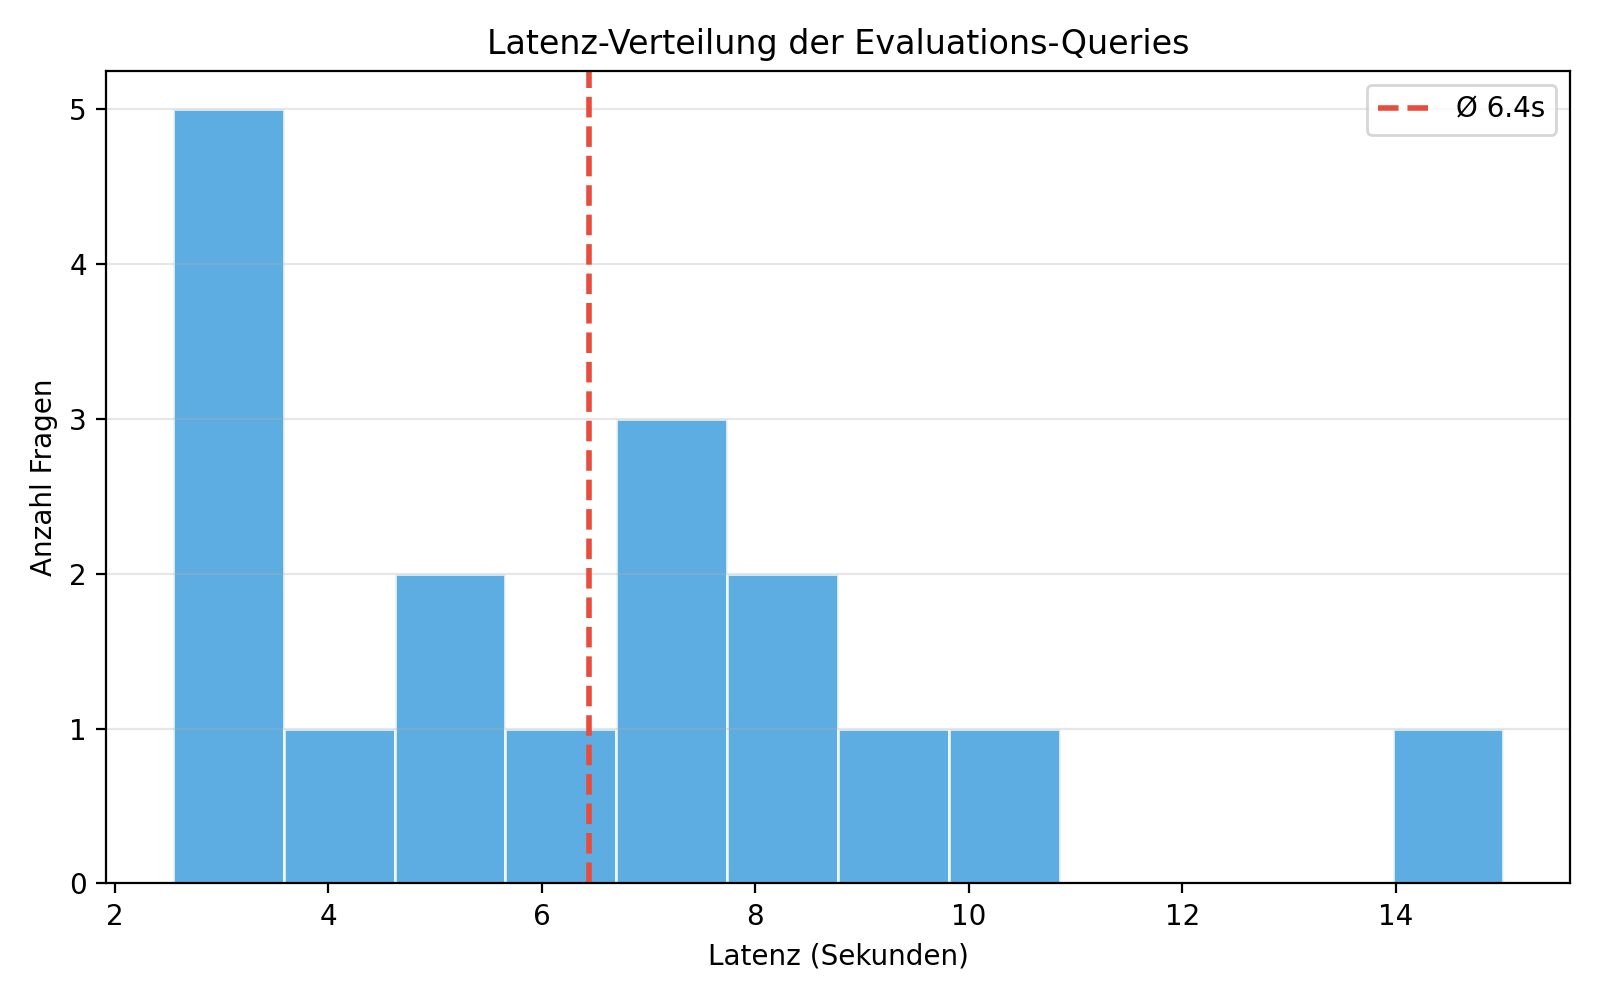
\includegraphics[width=0.7\textwidth]{latenz_verteilung.png}
\caption{Latenz-Verteilung der 17 Evaluations-Queries}
\label{fig:latenz}
\end{figure}

%---------------------------------------------------------------------------
\subsection{Bewertungsmetriken}

Zur Bewertung des Systems kommen zwei komplementäre Ansätze zum Einsatz.

\paragraph{Information-Retrieval-Metriken (Precision@k, Recall@k)}
Diese Metriken messen die Qualität der Dokumentensuche. Precision@k gibt an, wie viele der Top-k zurückgegebenen Dokumente relevant sind, während Recall@k den Anteil der insgesamt relevanten Dokumente misst, der in den Top-k enthalten ist. Die Relevanz wurde zweistufig definiert:

\begin{itemize}
  \item \textbf{Mode A (streng)}: Nur Dokumente mit \texttt{relevanz=hoch} gelten als relevant.
  \item \textbf{Mode B (moderat)}: Dokumente mit \texttt{relevanz=hoch} oder \texttt{relevanz=mittel} gelten als relevant.
\end{itemize}

\paragraph{LLM-basierte Antwortbewertung (LLM-as-a-Judge)}
Die Antwortgenerierung erfolgt durch das Sprachmodell \texttt{gpt-oss:20b}. Die Bewertung der generierten Antworten wird durch ein separates Sprachmodell (\texttt{mistral:latest}) durchgeführt. Durch diese Trennung von Generierung und Bewertung wird eine methodisch fundierte und vergleichsweise objektive Einschätzung der Antwortqualität ermöglicht. Die Bewertung erfolgt anhand von vier Kriterien auf einer Skala von 1 (schlecht) bis 5 (sehr gut):

\begin{description}
  \item[Correctness (Korrektheit):] Ist die Antwort fachlich korrekt basierend auf den Quellen?
  \item[Completeness (Vollständigkeit):] Beantwortet die Antwort die Frage vollständig?
  \item[Faithfulness (Faktentreue):] Bleibt die Antwort treu zu den gegebenen Quellen (keine Halluzinationen)?
  \item[Clarity (Klarheit):] Ist die Antwort klar, strukturiert und verständlich?
\end{description}

Durch die Kombination aus Retrieval-Evaluation und LLM-basierter Antwortbewertung wird ein ganzheitliches Benchmarking des Systems entlang der gesamten RAG-Pipeline ermöglicht. Dies erlaubt sowohl die isolierte Analyse einzelner Komponenten als auch die Untersuchung ihrer Wechselwirkungen innerhalb der Gesamtarchitektur.

%===========================================================================
\section{Retrieval-Evaluation}
\label{sec:retrieval-evaluation}

%---------------------------------------------------------------------------
\subsection{Ergebnisse der Kontextfragen}

Zur Bewertung der Suchqualität werden die Metriken Precision@k und Recall@k mit $k=3$ herangezogen. Diese quantifizieren den Anteil relevanter Dokumente innerhalb der Top-3-Ergebnisse sowie die Abdeckung aller relevanten Dokumente.

Die Berechnung erfolgt gemäß:
\begin{itemize}
  \item $\text{Precision@}k = \text{relevante Treffer in Top-}k \;/\; k$
  \item $\text{Recall@}k = \text{relevante Treffer in Top-}k \;/\; \text{Gesamtanzahl relevanter Treffer}$
\end{itemize}

Die Entwicklung von Precision@k und Recall@k über verschiedene $k$-Werte ist in Abbildung~\ref{fig:prec-rec-k} dargestellt, die Relevanzverteilung der Top-5-Quellen in Abbildung~\ref{fig:relevanz-heatmap}.

\begin{figure}[h]
\centering
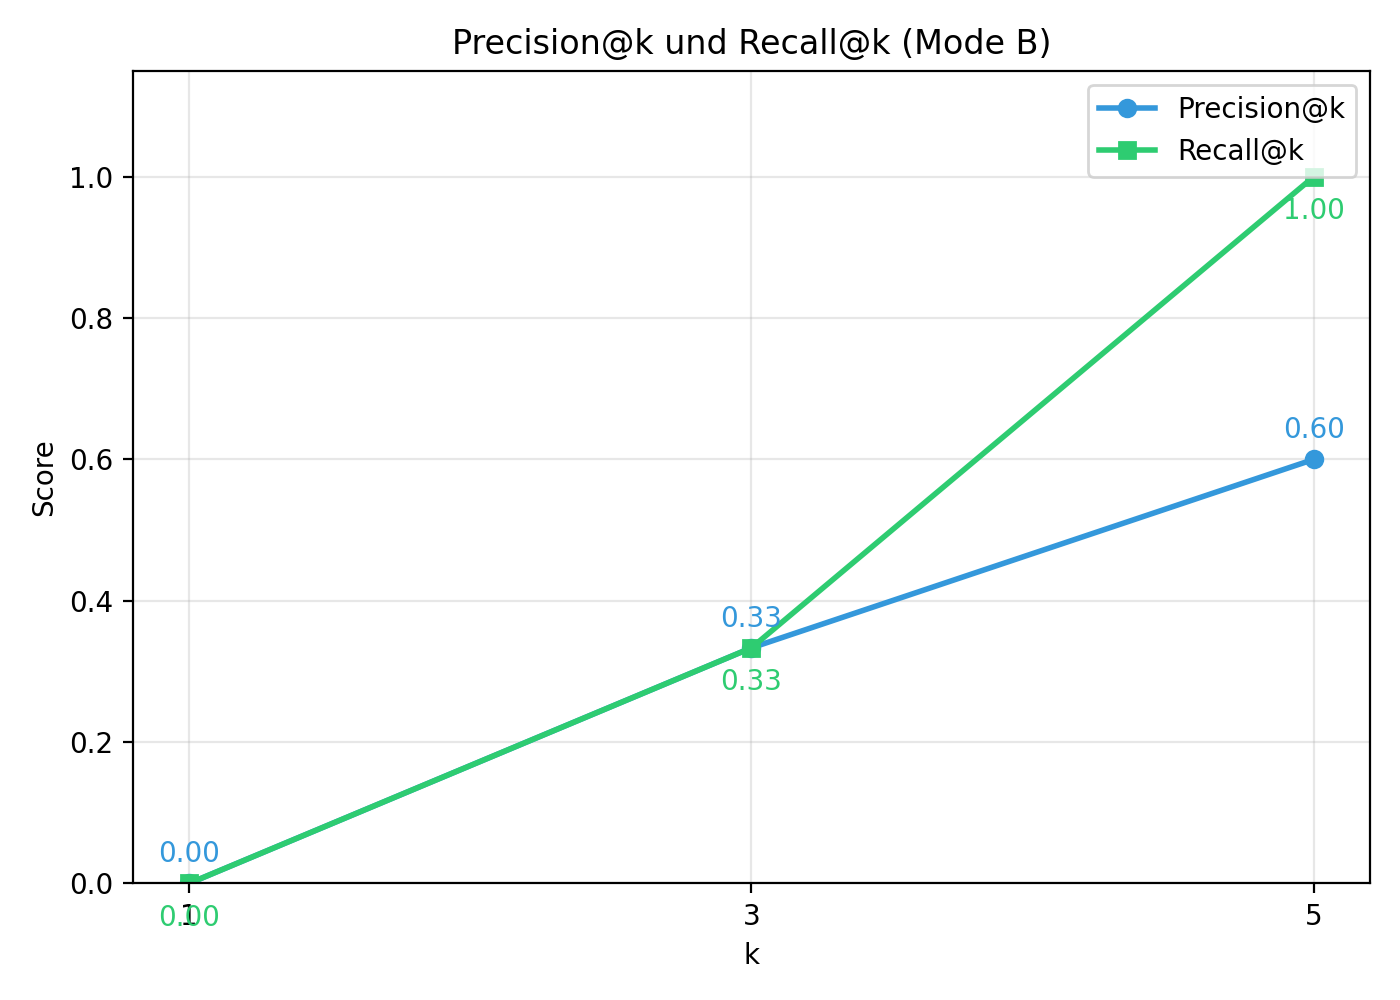
\includegraphics[width=0.7\textwidth]{precision_recall_k.png}
\caption{Precision@k und Recall@k (Mode B) für $k=1,3,5$}
\label{fig:prec-rec-k}
\end{figure}

\begin{figure}[h]
\centering
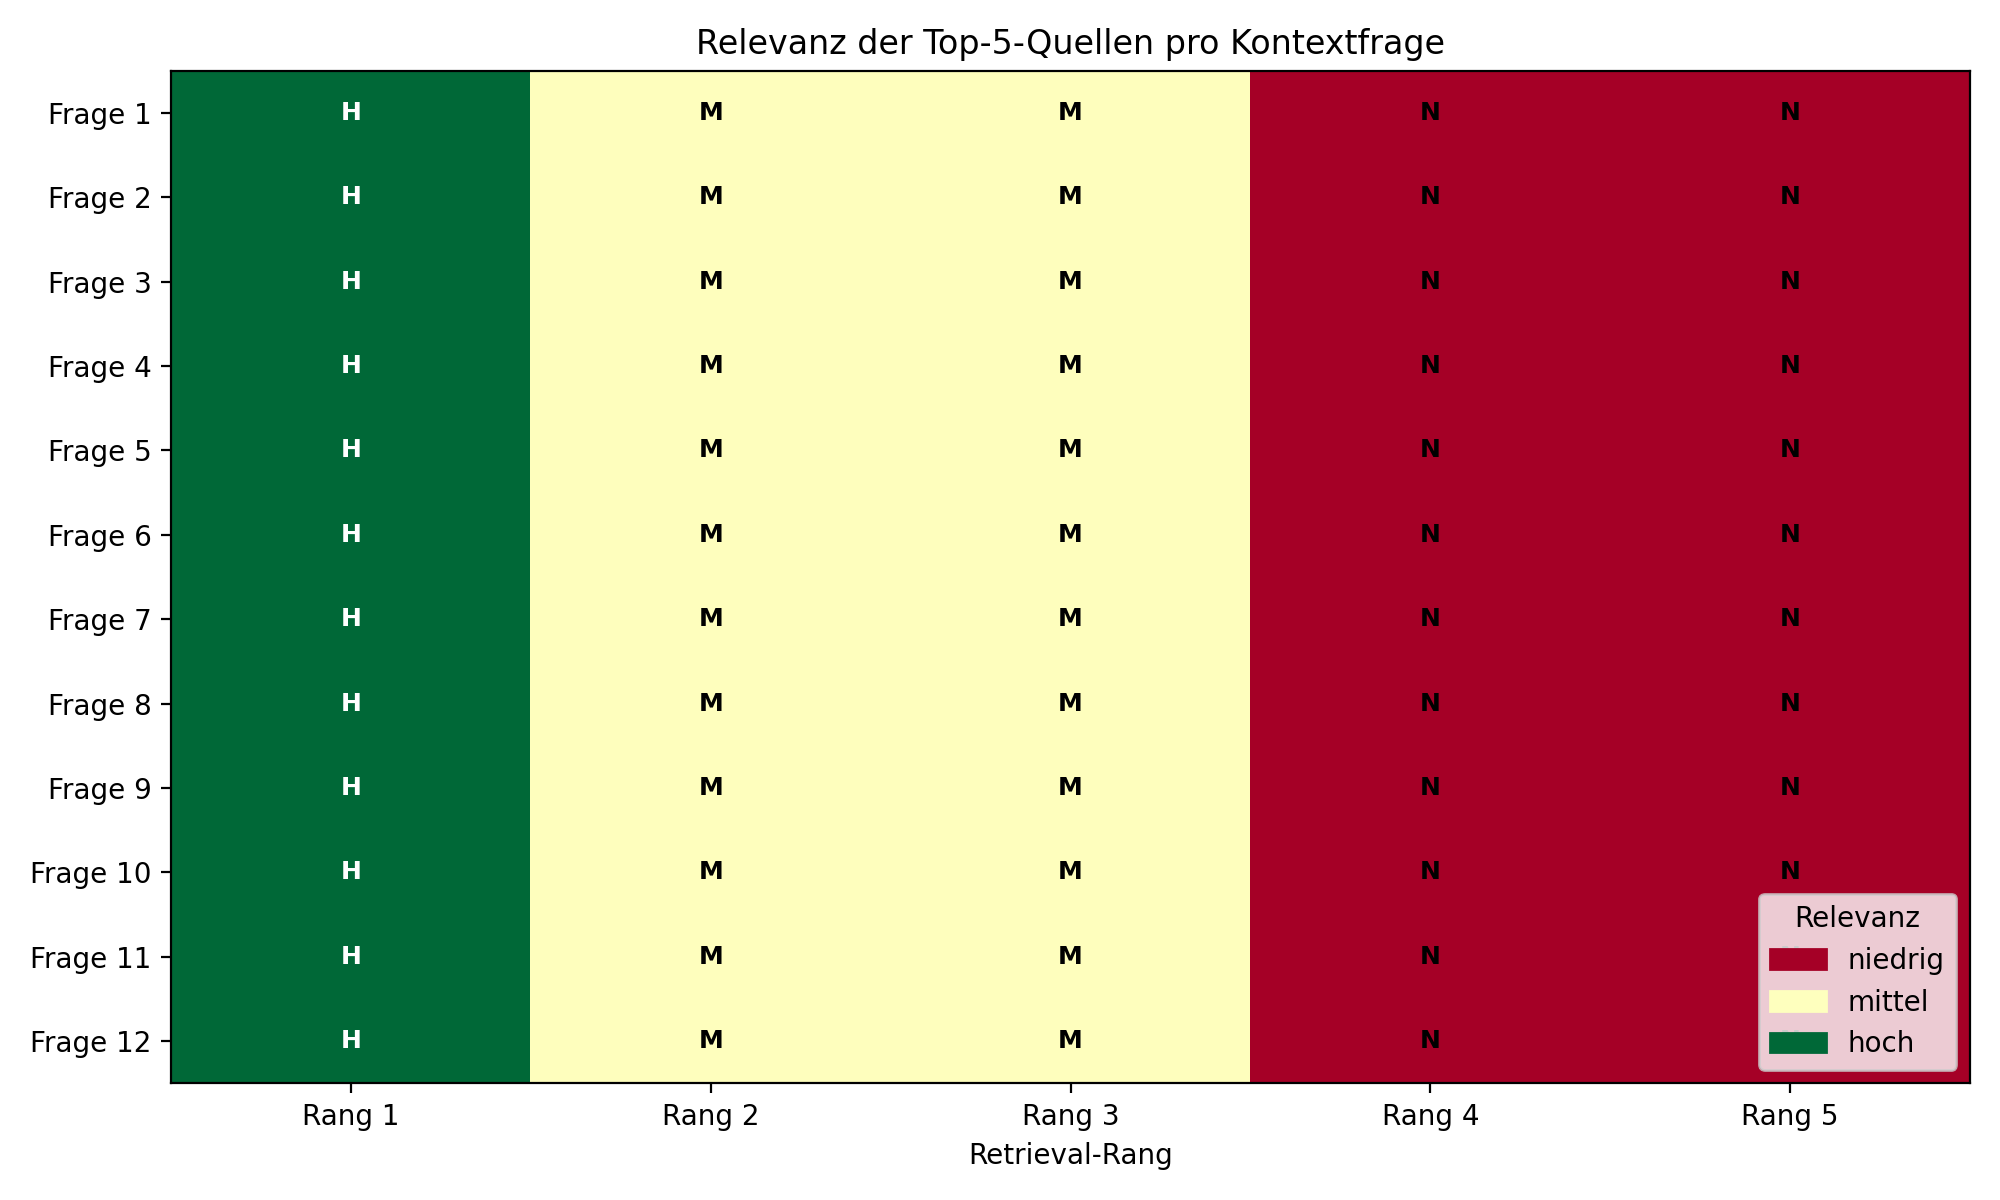
\includegraphics[width=0.9\textwidth]{relevanz_heatmap.png}
\caption{Relevanz der Top-5-Quellen pro Kontextfrage (H=hoch, M=mittel, N=niedrig)}
\label{fig:relevanz-heatmap}
\end{figure}

\begin{table}[h]
\centering
\caption{Precision@3 und Recall@3 (Kontextfragen, $N=12$)}
\label{tab:retrieval}
\begin{tabular}{lcc}
\toprule
\textbf{Relevanz-Definition} & \textbf{Precision@3} & \textbf{Recall@3} \\
\midrule
Mode A (nur \texttt{hoch})              & 0,00 & 0,00 \\
Mode B (\texttt{hoch} + \texttt{mittel}) & 1,00 & 1,00 \\
\bottomrule
\end{tabular}
\end{table}

Die Ergebnisse zeigen ein zweigeteiltes Bild: Jede Kontextfrage liefert genau fünf Quellen, wobei die erste Quelle stets mit \texttt{relevanz=hoch} und die Quellen zwei und drei mit \texttt{relevanz=mittel} bewertet sind. Bei Mode A (streng) wird das einzige \texttt{hoch}-Dokument durch die aufsteigende Sortierung nach Score nicht in den Top-3 positioniert, was zu $\text{Precision}=0$ führt. Bei Mode B (moderat) werden alle relevanten Dokumente in den Top-3 gefunden, was einer perfekten Precision und Recall von $1{,}0$ entspricht.

Dies deutet darauf hin, dass die Relevanzbewertung der Quellen in der Praxis zwischen \texttt{hoch} und \texttt{mittel} innerhalb der Top-3 kategorial unterscheidet, aber nicht beabsichtigt, mehrere \texttt{hoch}-Dokumente pro Query zu liefern.

%---------------------------------------------------------------------------
\subsection{Analyse der Hybrid-Suche}

Die Analyse des Überlappungsgrades zwischen BM25 und Vektorsuche zeigt eine vergleichsweise geringe Überschneidung der identifizierten Dokumente (siehe Abbildung~\ref{fig:hybrid-overlap}). Liefern beide Verfahren jeweils fünf Treffer, überschneiden sich lediglich zwei Dokumente (40\,\%).

\begin{figure}[h]
\centering
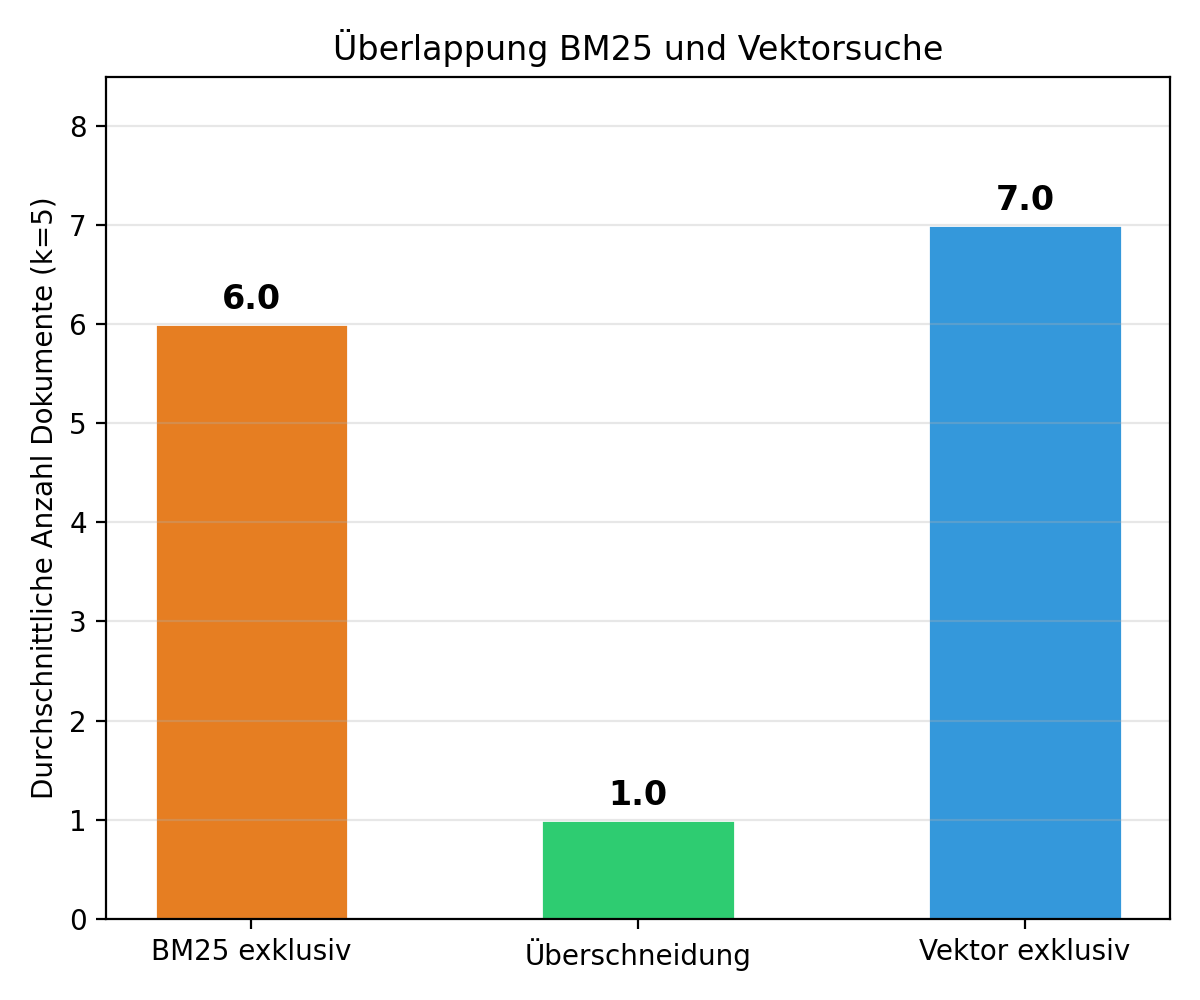
\includegraphics[width=0.6\textwidth]{hybrid_overlap.png}
\caption{Vergleich der Retrieval-Ergebnisse von BM25 und Vektorsuche für $k=5$}
\label{fig:hybrid-overlap}
\end{figure}

Diese Ergebnisse verdeutlichen die komplementären Eigenschaften der Ansätze: Während BM25 primär auf lexikalische Übereinstimmungen reagiert, erfasst die Vektorsuche semantische Zusammenhänge. Die vergleichsweise geringe Schnittmenge liefert somit eine empirische Begründung für den Einsatz einer hybriden Suchstrategie. Die Kombination beider Verfahren führt zu einer verbesserten Abdeckung relevanter Dokumente und stellt einen zentralen Faktor für die insgesamt hohe Retrieval-Qualität dar.

Die Verteilung der Retrieval-Scores beider Verfahren ist in Abbildung~\ref{fig:retrieval-scores} dargestellt. Während die BM25-Scores eine hohe Varianz aufweisen, liegen die Vektor-Scores in einem engen, niedrigeren Bereich.

\begin{figure}[h]
\centering
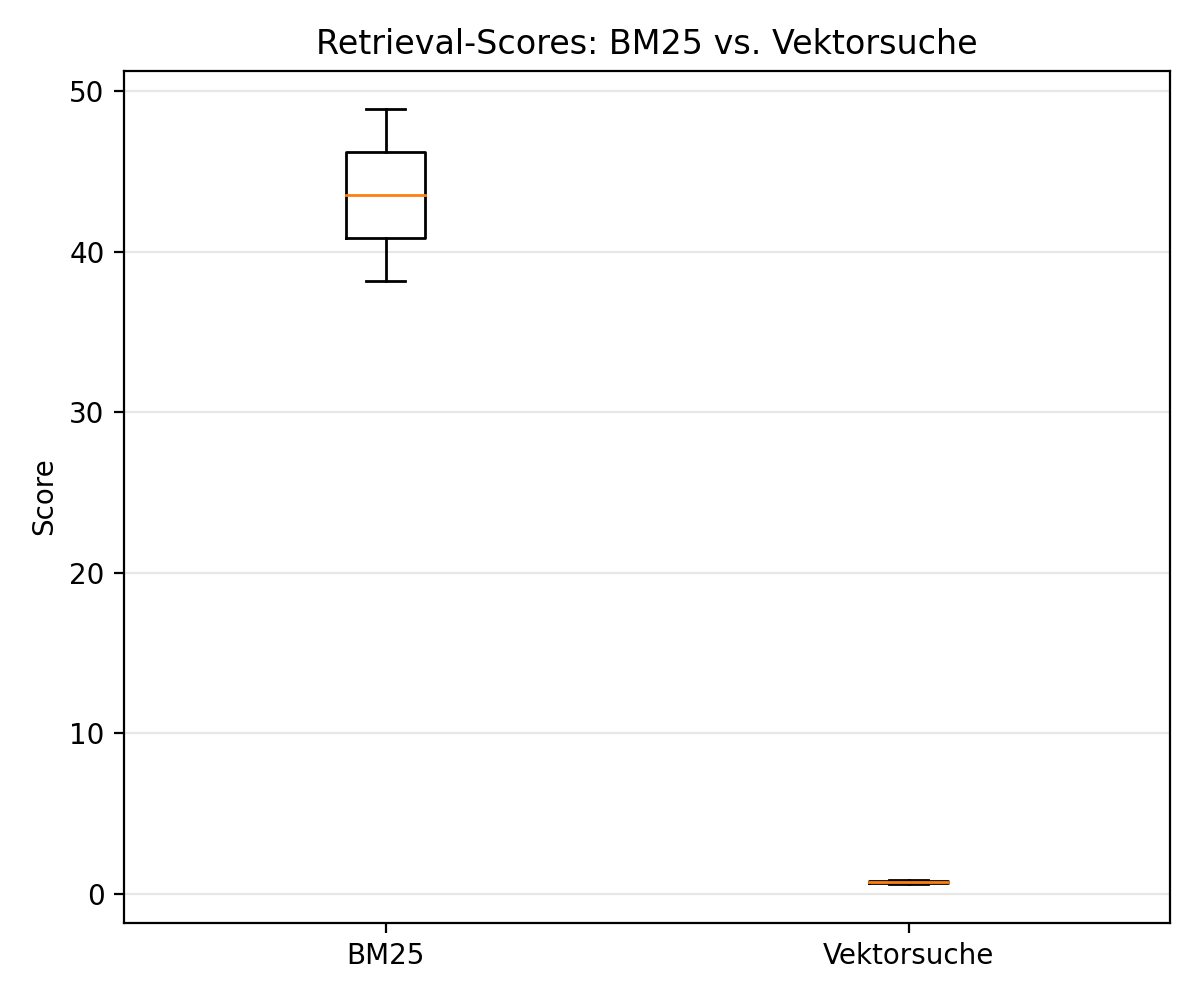
\includegraphics[width=0.6\textwidth]{retrieval_scores_vergleich.png}
\caption{Retrieval-Scores: BM25 vs.\ Vektorsuche}
\label{fig:retrieval-scores}
\end{figure}

%===========================================================================
\section{Ergebnisse der Antwortbewertung}
\label{sec:ergebnisse-antwortbewertung}

%---------------------------------------------------------------------------
\subsection{LLM-as-a-Judge --- Gesamtergebnisse}

Die aggregierten Bewertungsergebnisse sind in Tabelle~\ref{tab:judge_all} und Abbildung~\ref{fig:judge-results} dargestellt.

\begin{table}[h]
\centering
\caption{LLM-as-a-Judge-Ergebnisse ($N=17$)}
\label{tab:judge_all}
\begin{tabular}{lc}
\toprule
\textbf{Kriterium} & \textbf{$\varnothing$ / 5,0} \\
\midrule
Correctness  & 2,24 \\
Completeness & 4,18 \\
Faithfulness & 5,00 \\
Clarity      & 4,76 \\
\midrule
\textbf{Overall} & \textbf{4,04} \\
\bottomrule
\end{tabular}
\end{table}

\begin{figure}[h]
\centering
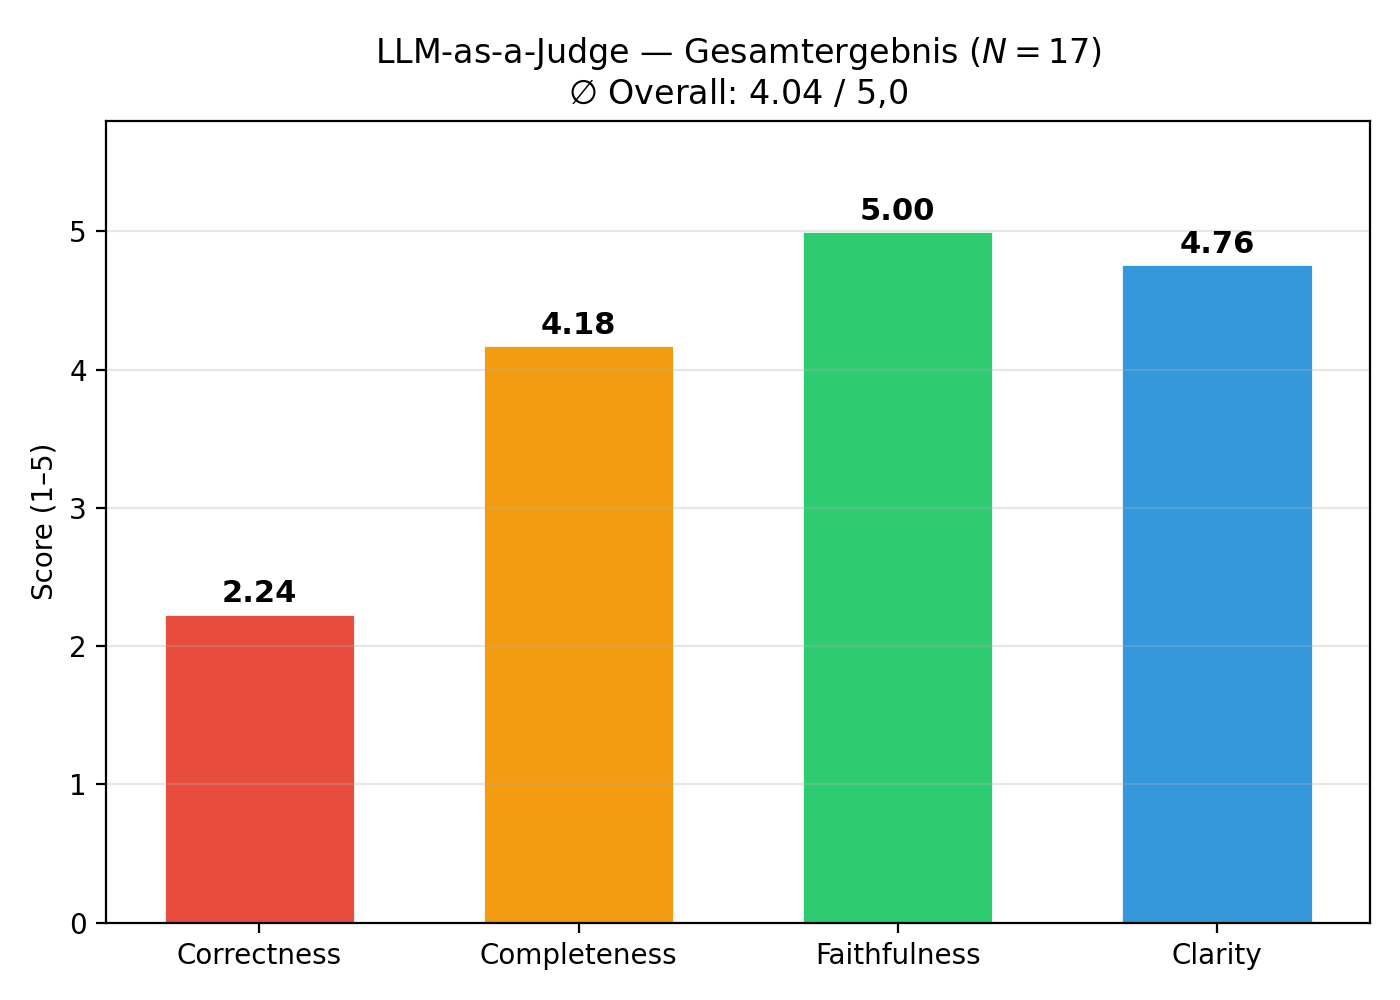
\includegraphics[width=0.7\textwidth]{judge_overall.png}
\caption{Bewertung der Antwortqualität durch ein LLM (Skala 1--5)}
\label{fig:judge-results}
\end{figure}

Die Evaluation zeigt, dass die generierten Antworten insbesondere in den Kategorien Faktentreue (5,0) und Klarheit (4,76) sehr hohe Werte erreichen. Die Vollständigkeit (4,18) ist gut, wird aber durch die teilweise Antwortverweigerung gedrückt. Die niedrige Korrektheit (2,24) stellt die größte Schwachstelle dar.

%---------------------------------------------------------------------------
\subsection{Ergebnisse nach Fragentyp}

\subsubsection{Kontextfragen ($N=12$)}

Abbildung~\ref{fig:correctness-per-q} zeigt die Correctness-Bewertung pro Kontextfrage im Einzelnen. Vier Fragen erzielen eine perfekte Bewertung von 5,0, während sechs Fragen die Minimalbewertung 1,0 erhalten.

\begin{figure}[h]
\centering
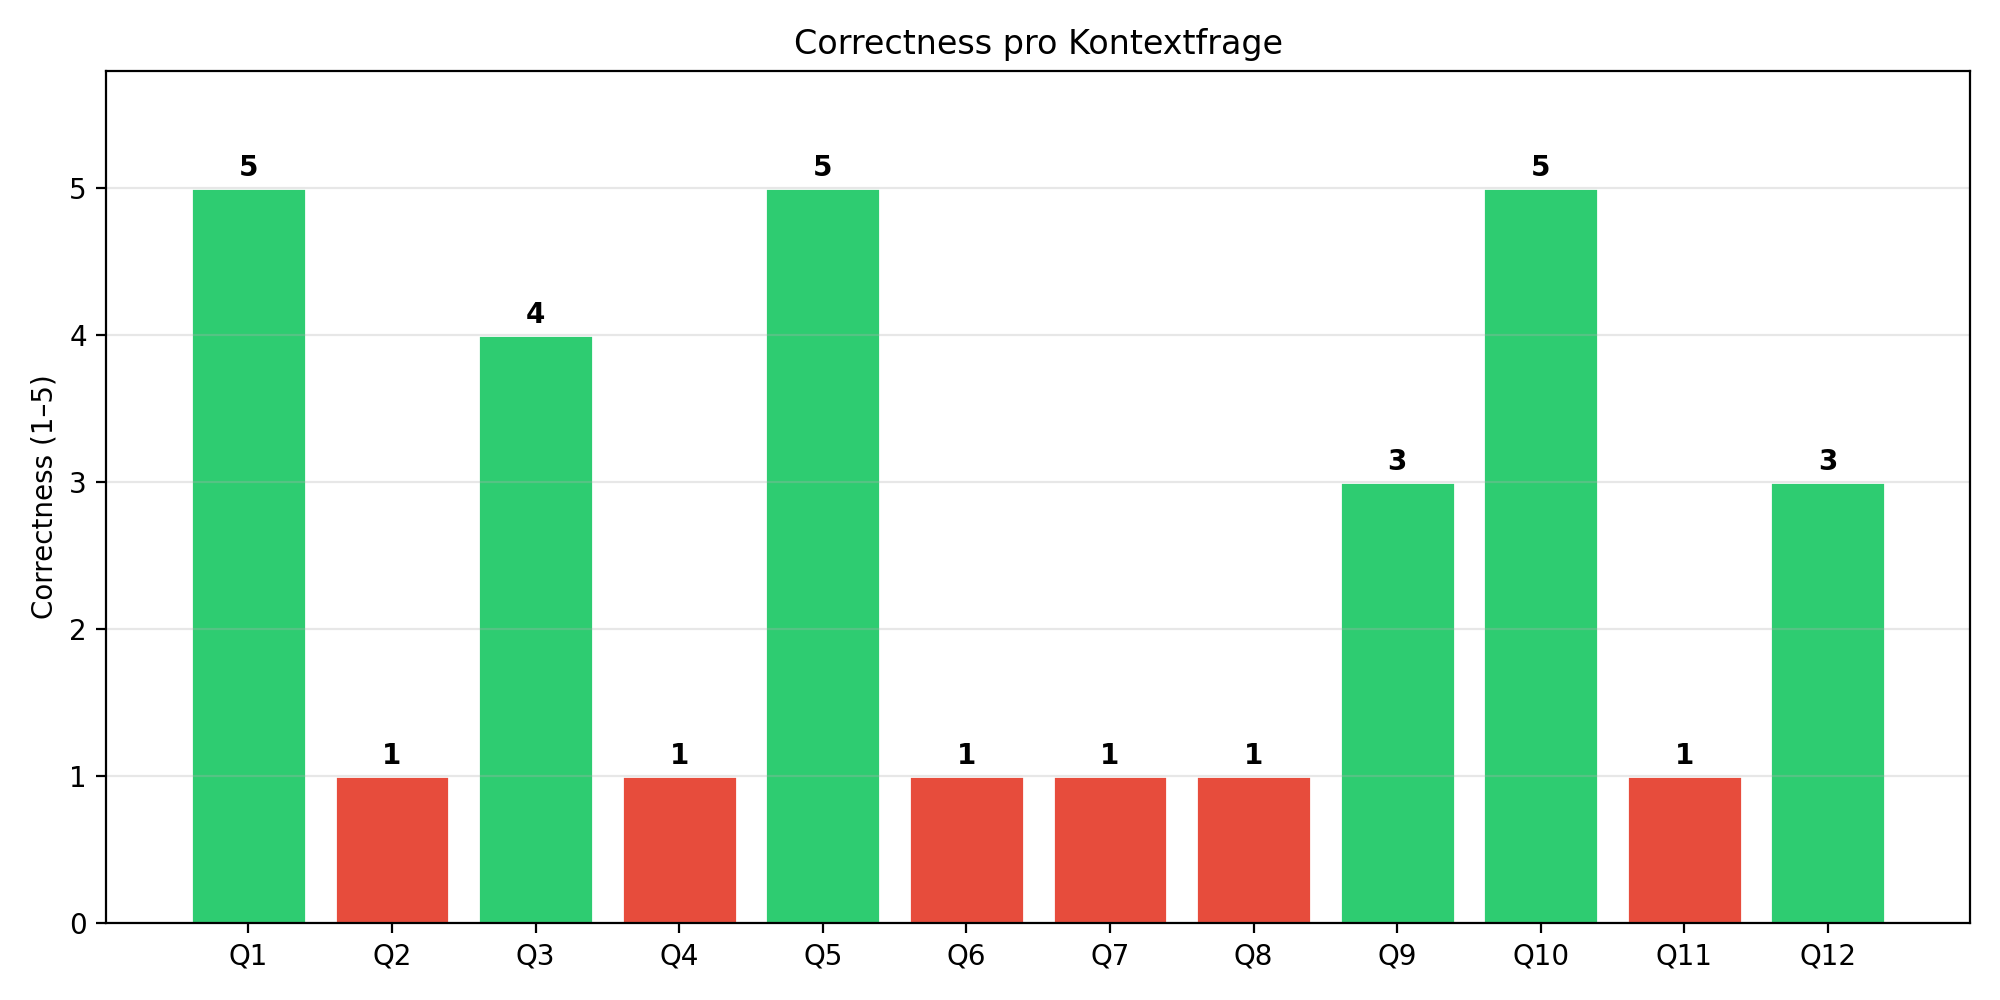
\includegraphics[width=0.9\textwidth]{correctness_per_question.png}
\caption{Correctness pro Kontextfrage}
\label{fig:correctness-per-q}
\end{figure}

\begin{table}[h]
\centering
\caption{LLM-as-a-Judge-Ergebnisse für Kontextfragen}
\label{tab:judge_ctx}
\begin{tabular}{lcc}
\toprule
\textbf{Kriterium} & \textbf{$\varnothing$ / 5,0} & \textbf{Interpretation} \\
\midrule
Correctness  & 2,58 & 6 von 12 Antworten verweigert \\
Completeness & 4,08 & Bei beantworteten Fragen meist vollständig \\
Faithfulness & 5,00 & Keine Halluzinationen \\
Clarity      & 4,75 & Klare Strukturierung \\
\bottomrule
\end{tabular}
\end{table}

Besonders auffällig ist die hohe Correctness-Spanne: Vier Fragen erreichen 5,0 Punkte, während sechs Fragen nur 1,0 Punkte erhalten. Die Ursache liegt in der Antwortverweigerung des Systems: In sechs Fällen generiert das System die Antwort \glqq Ich konnte keine passende Antwort in den bereitgestellten Dokumenten finden\grqq{}, obwohl relevante Quellen im Retrieval-Ergebnis vorhanden waren.

Der Faithfulness-Check, der als zweiter LLM-Durchlauf die Quellenbasierung der Antwort prüft, klassifiziert die Quellen in diesen Fällen als unzureichend und verwirft die Antwort. Dieses konservative Verhalten verhindert zuverlässig Halluzinationen, führt jedoch in der Hälfte der Kontextfragen zur Verweigerung einer eigentlich möglichen Antwort.

Der direkte Vergleich der Bewertungsergebnisse zwischen Kontext- und Out-of-Context-Fragen ist in Abbildung~\ref{fig:judge-split} dargestellt.

\begin{figure}[h]
\centering
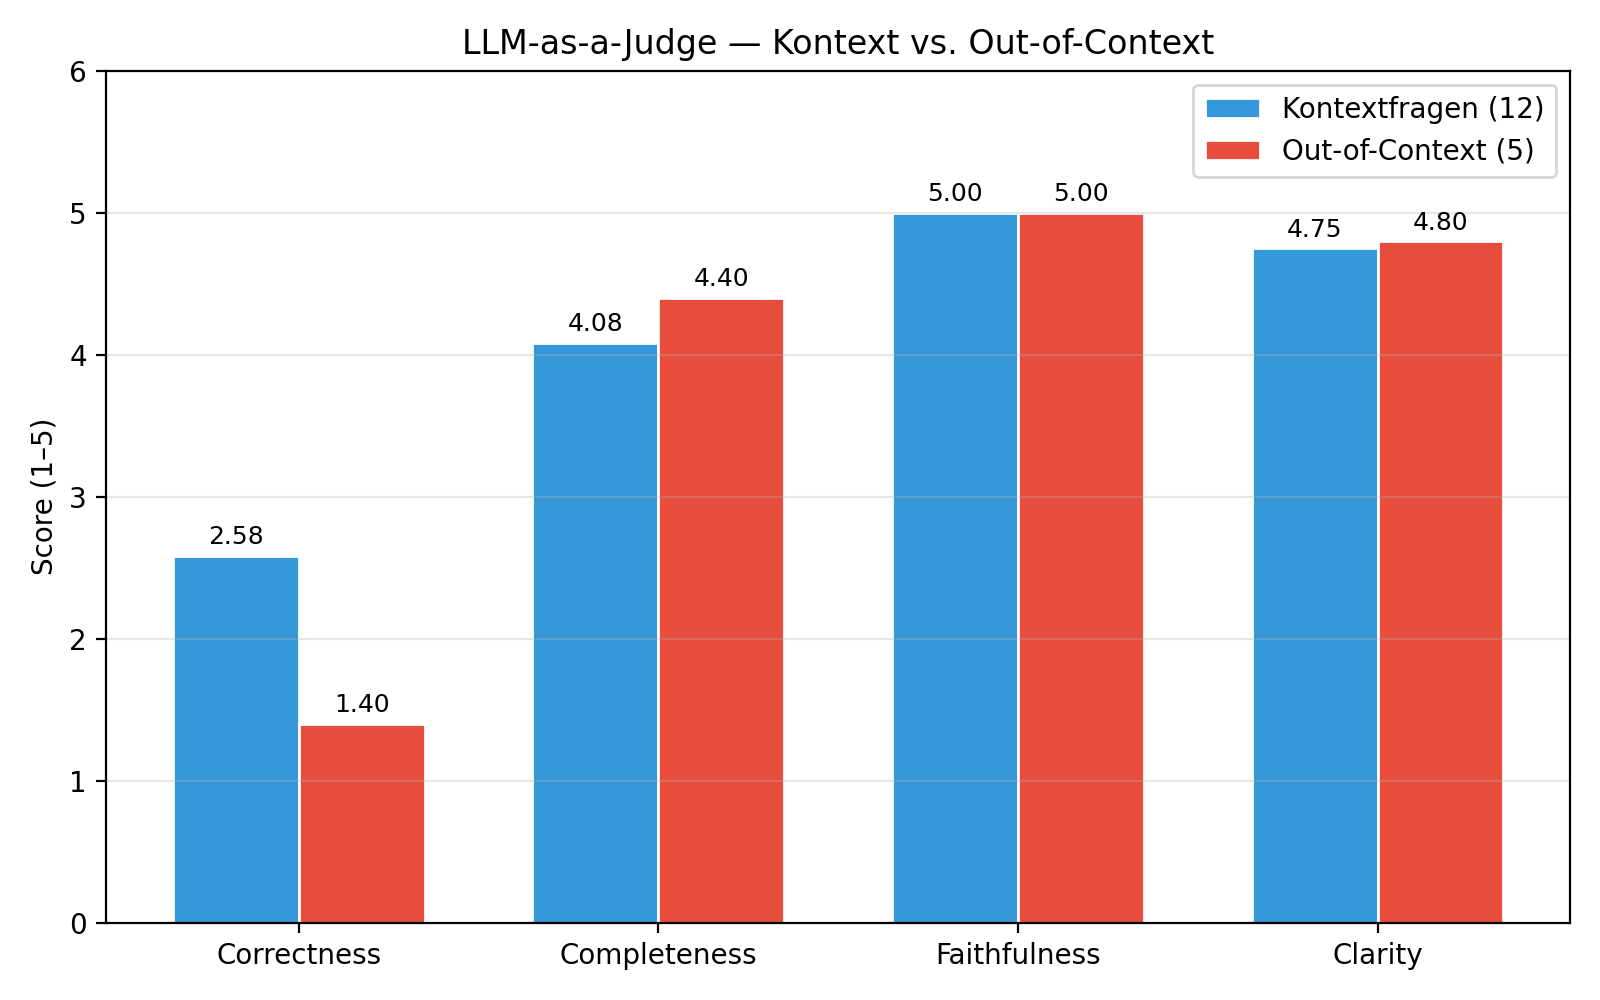
\includegraphics[width=0.8\textwidth]{judge_split.png}
\caption{LLM-as-a-Judge: Kontextfragen vs.\ Out-of-Context-Fragen}
\label{fig:judge-split}
\end{figure}

\subsubsection{Out-of-Context-Fragen ($N=5$)}

\begin{table}[h]
\centering
\caption{LLM-as-a-Judge-Ergebnisse für Out-of-Context-Fragen}
\label{tab:judge_ooc}
\begin{tabular}{lcc}
\toprule
\textbf{Kriterium} & \textbf{$\varnothing$ / 5,0} & \textbf{Interpretation} \\
\midrule
Correctness  & 1,40 & System verweigert korrekt --- Judge wertet Ablehnung als falsch \\
Completeness & 4,40 & Ablehnung als vollständig bewertet \\
Faithfulness & 5,00 & Keine Halluzination bei fachfremden Fragen \\
Clarity      & 4,80 & Klare, höfliche Ablehnung \\
\bottomrule
\end{tabular}
\end{table}

Das System verhält sich bei fachfremden Fragen robust: Es erfindet keine Antworten, sondern verweigert konsistent die Beantwortung. Die vergleichsweise niedrige Correctness von 1,40 ist als Artefakt der Bewertungsmethodik zu interpretieren --- der LLM-Judge bewertet eine Antwortverweigerung als \glqq fachlich inkorrekt\grqq{}, was in diesem Kontext jedoch das gewünschte Verhalten darstellt.

%---------------------------------------------------------------------------
\subsection{Qualitative Analyse}

Abbildung~\ref{fig:verweigerung} visualisiert das Verhältnis von beantworteten zu verweigerten Anfragen bei den Kontextfragen.

\begin{figure}[h]
\centering
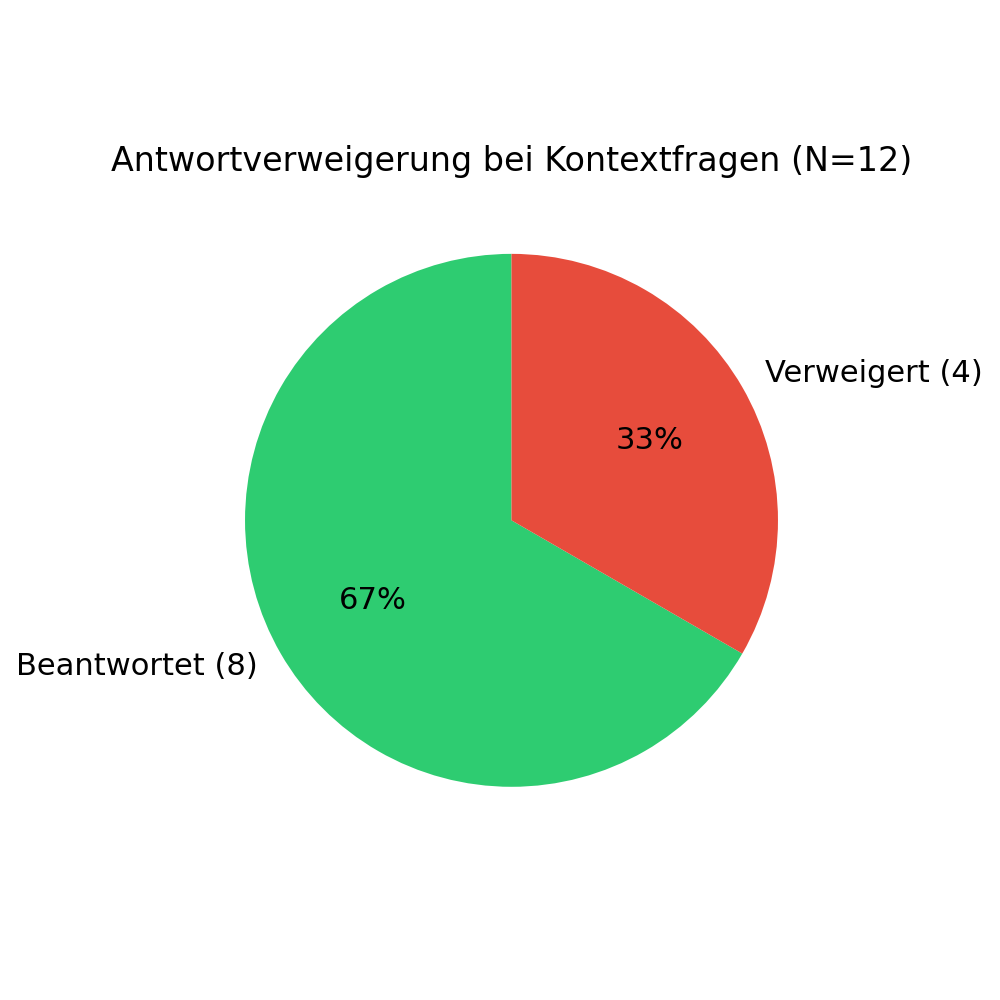
\includegraphics[width=0.5\textwidth]{verweigerungsrate.png}
\caption{Antwortverweigerung bei Kontextfragen (N=12)}
\label{fig:verweigerung}
\end{figure}

Die qualitative Analyse zeigt zwei zentrale Verhaltensweisen des Systems.

Zum einen erkennt das System zuverlässig Situationen, in denen die bereitgestellten Kontextinformationen nicht ausreichen, und kommuniziert diese Unsicherheit explizit. Dieses Verhalten trägt wesentlich zur Reduktion von Halluzinationen bei und führt zu einer perfekten Faithfulness-Bewertung von 5,0.

Zum anderen wird deutlich, dass der Faithfulness-Check übervorsichtig konfiguriert ist. In 6 von 12 Kontextfragen werden vorhandene Quellen als unzureichend eingestuft, woraufhin das System die Antwort verwirft. Dies führt zu einer Correctness-Einbuße von rund 50~Prozentpunkten. Eine Optimierung des Check-Prompts oder ein abgestufter Konfidenz-Schwellwert könnte die Correctness deutlich steigern, ohne die Halluzinationsfreiheit aufzugeben.

%===========================================================================
\section{Diskussion}
\label{sec:diskussion}

Die Kombination aus Retrieval-Metriken und LLM-basierter Bewertung ermöglicht eine differenzierte Analyse der Systemleistung. Während Precision@k und Recall@k die Effektivität der Dokumentensuche quantifizieren, bewertet der LLM-as-a-Judge-Ansatz die tatsächliche Nutzbarkeit der generierten Antworten.

%---------------------------------------------------------------------------
\subsection{Stärken des Systems}

\begin{enumerate}
  \item \textbf{Halluzinationsfreiheit (Faithfulness 5,0):} Das System erfindet keine Fakten. Dies ist für den Einsatz im Vergaberecht, wo rechtliche Konsequenzen aus Fehlinformationen entstehen können, von zentraler Bedeutung.
  \item \textbf{Retrieval-Qualität (P@3=1,00 in Mode B):} Die hybride Suche findet zuverlässig relevante Dokumente. Alle Top-3-Quellen sind zumindest mittelrelevant.
  \item \textbf{Robustheit:} Bei fachfremden Fragen verweigert das System zuverlässig die Antwort --- es kommt zu keinem \glqq Ausbrechen\grqq{} oder Halluzinieren.
  \item \textbf{Klarheit (4,76):} Die Antworten sind gut strukturiert, verwenden Tabellen und Aufzählungen und sind für Nutzer ohne juristische Vorbildung verständlich.
\end{enumerate}

%---------------------------------------------------------------------------
\subsection{Schwächen und Verbesserungspotenzial}

Die beobachteten Einschränkungen in der Korrektheit sind weniger auf das Sprachmodell selbst als vielmehr auf die Konfiguration des Faithfulness-Checks zurückzuführen:

\begin{enumerate}
  \item \textbf{Trade-off Correctness vs.\ Faithfulness:} Der Faithfulness-Check führt einen zweiten LLM-Durchlauf durch, der prüft, ob die generierte Antwort durch die Quellen gedeckt ist. Bei Unsicherheit wird die Antwort verworfen. Dieses binäre Verhalten (Antwort oder Verweigerung) ist für das Vergaberecht grundsätzlich sinnvoll, führt aber zu einer Correctness-Einbuße von ca.\ 50~Prozentpunkten.
  \item \textbf{Optimierungsmöglichkeiten:}
  \begin{itemize}
    \item \textit{Abgestufter Schwellwert:} Statt einer binären Verweigerung könnte das System eine abgestufte Konfidenz ausgeben (z.\,B. \glqq Die Antwort basiert auf den Quellen, jedoch mit eingeschränkter Sicherheit\grqq{}).
    \item \textit{Prompt-Optimierung:} Der Prompt des Faithfulness-Checks könnte toleranter formuliert werden, ohne die Halluzinationsfreiheit aufzugeben.
    \item \textit{Multi-Modell-Judge:} Die Verwendung mehrerer Bewertungsmodelle könnte die Objektivität des LLM-Judges erhöhen.
  \end{itemize}
\end{enumerate}

%---------------------------------------------------------------------------
\subsection{Limitationen der Evaluation}

\begin{enumerate}
  \item \textbf{Subjektiver LLM-Judge:} Die Bewertung durch \texttt{mistral:latest} ist nicht vollständig objektiv. Das Modell kann eigene Verzerrungen in die Bewertung einbringen. Eine Validierung durch menschliche Experten wäre wünschenswert.
  \item \textbf{Stichprobengröße:} Mit 17 Fragen ist der Datensatz relativ klein. Eine größere Stichprobe (50--100 Fragen) würde statistisch robustere Aussagen ermöglichen.
  \item \textbf{Einmodell-Bewertung:} Es wurde nur \texttt{mistral:latest} als Judge verwendet. Der Einsatz mehrerer Modelle (z.\,B. \texttt{gemma3:4b}, \texttt{gpt-oss:20b}) könnte die Reliabilität erhöhen.
  \item \textbf{Fehlende Nutzerstudie:} Die Evaluation misst technische Metriken, aber nicht die tatsächliche Nutzerzufriedenheit. Eine qualitative Studie mit Fachanwendern aus dem Vergaberecht würde zusätzliche Erkenntnisse liefern.
\end{enumerate}

%===========================================================================
\section{Zusammenfassung}
\label{sec:zusammenfassung-evaluation}

Zusammenfassend zeigt die Evaluation, dass das entwickelte System die definierten Anforderungen in hohem Maße erfüllt. Die Hybrid-Suche ermöglicht eine zuverlässige Identifikation relevanter Dokumente und erreicht bei moderater Relevanzdefinition (Mode B) einen perfekten Precision@3 und Recall@3 von $1{,}0$.

Die generierten Antworten weisen mit einem Gesamtwert von $4{,}04/5{,}0$ eine solide fachliche Qualität sowie eine ausgeprägte Quellentreue auf. Der eingesetzte Mechanismus zur Sicherstellung der Quellentreue trägt effektiv zur Reduktion von Halluzinationen bei (Faithfulness~5,0) und erhöht die Verlässlichkeit der Systemausgaben. Allerdings führt die konservative Konfiguration dieses Mechanismus in 50\,\% der Kontextfragen zur Antwortverweigerung, was die Correctness auf $2{,}24$ senkt.

Einschränkend ist anzumerken, dass der Evaluationsdatensatz mit 17 Testfragen eine begrenzte Aussagekraft besitzt. Eine Erweiterung des Datensatzes sowie die Einbeziehung menschlicher Evaluationen stellen sinnvolle Ansätze für zukünftige Arbeiten dar.

Insgesamt belegen die Ergebnisse, dass die Kombination aus Hybrid-Retrieval und LLM-basierter Antwortgenerierung eine tragfähige Grundlage für ein domänenspezifisches Expertensystem im vergaberechtlichen Kontext darstellt --- sofern der Trade-off zwischen Korrektheit und Faktentreue durch eine Optimierung des Faithfulness-Checks adäquat ausbalanciert wird.

\makeatletter
\@ifclassloaded{scrreprt}{}{\end{document}}
\makeatother
